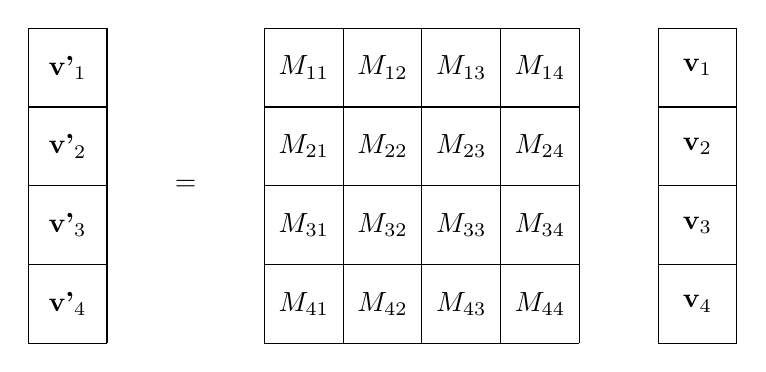
\begin{tikzpicture}

    \draw foreach \x in {0,...,1} {(-3+\x,0) -- (-3+\x,4)};
    \draw foreach \x in {0,...,4} {(-3,\x) -- (-2,\x)};
    
    \foreach \x in {0,...,3} {
        \node at (-2.5,\x+0.5) {$\textbf{v'}_{\fpeval{4 - \x}}$};
    }
    
    \node at (-1,2) {$=$};

    \draw foreach \x in {0,...,4} {(\x,0) -- (\x,4) (0,\x) -- (4,\x)};

    \foreach \x in {0,...,3} {
        \foreach \y in {0,...,3} {
            \node at (\x+0.5,\y+0.5) {$M_{\fpeval{4 - \y} \fpeval{\x + 1}}$};
        }
    }

    \draw foreach \x in {0,...,1} {(5+\x,0) -- (5+\x,4)};
    \draw foreach \x in {0,...,4} {(5,\x) -- (6,\x)};
    
    \foreach \x in {0,...,3} {
        \node at (5.5,\x+0.5) {$\textbf{v}_{\fpeval{4 - \x}}$};
    }

\end{tikzpicture}
